\normaltrue \difficilefalse \tdifficilefalse
\correctionfalse

%\UPSTIidClasse{11} % 11 sup, 12 spé
%\newcommand{\UPSTIidClasse}{12}

\exer{Treuil de levage $\star$ \label{CIN:03:C2:06:38}}
\marginnote{\textit{D'après ressources Pole Chateaubriand -- Joliot-Curie.}}
\setcounter{question}{0}\marginnote{\xpComp{CIN}{03}}%\UPSTIcompetence[2]{A3-05}
%\UPSTIcompetence[2]{C2-06}
\index{Compétence C2-06}\index{Compétence CIN-03}
%\index{Train d'engrenages simple}
\ifcorrection
\else
\marginnote{\textbf{Pas de corrigé pour cet exercice.}}
\fi

\ifprof
\else
On s’intéresse à un treuil dont le modèle cinématique est donné ci-dessous.
\begin{marginfigure}
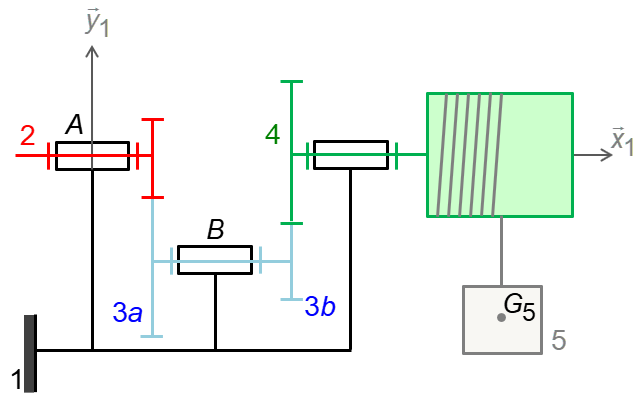
\includegraphics[width=\linewidth]{38_01}
\end{marginfigure}

On note $Z_2$ le nombre de dents de la roue dentée de l'arbre 2. On note l'arbre intermédiaire 3 et $Z_{3a}$ et $Z_{3b}$ les nombres de dents de ses deux roues dentées. On note $R$ le rayon du tambour 4 sur lequel s’enroule sans glisser un câble et $Z_4$ le nombre de dents de sa roue dentée.
\fi


\question{Déterminer la relation entre $v_{51}$ la vitesse de déplacement de la charge par rapport au bâti et $\omega_{21}$ la vitesse de rotation du moteur.}
\ifprof
\else
\fi

\question{On note $J_2$, $J_3$, $J_4$ l'inertie des pièces 2, 3 et 5. On note $M_5$ la masse du solide 5. Donner la masse équivalente ramenée << à la translation >> de la masse. Donner l'inertie équivalente ramenée à l'arbre d'entrée 2.}
\ifprof ~\\

\else
\fi


\ifprof
\else

\marginnote{Corrigé voir \ref{CIN:03:C2:06:38}.}

\fi